\documentclass[10pt]{article} % Font size - 10pt, 11pt or 12pt

\usepackage[hmargin=1.25cm, vmargin=1.5cm]{geometry} % Document margins

\usepackage{graphicx}
\usepackage{amsmath}
\usepackage{listings}

\usepackage[usenames,dvipsnames]{xcolor} % Allows the definition of hex colors

% Fonts and tweaks for XeLaTeX
\usepackage{fontspec,xltxtra,xunicode}
\defaultfontfeatures{Mapping=tex-text}
%\setmonofont[Scale=MatchLowercase]{Andale Mono}

% Colors for links, text and headings
\usepackage{hyperref}
\definecolor{linkcolor}{HTML}{506266} % Blue-gray color for links
\definecolor{shade}{HTML}{F5DD9D} % Peach color for the contact information box
\definecolor{text1}{HTML}{2b2b2b} % Main document font color, off-black
\definecolor{headings}{HTML}{701112} % Dark red color for headings
% Other color palettes: shade=B9D7D9 and linkcolor=A40000; shade=D4D7FE and linkcolor=FF0080

\hypersetup{colorlinks,breaklinks, urlcolor=linkcolor, linkcolor=linkcolor} % Set up links and colors

\usepackage{fancyhdr}
\pagestyle{fancy}
\fancyhf{}
% Headers and footers can be added with the \lhead{} \rhead{} \lfoot{} \rfoot{} commands
% Example footer:
%\rfoot{\color{headings} {\sffamily Last update: \today}. Typeset with Xe\LaTeX}

\renewcommand{\headrulewidth}{0pt} % Get rid of the default rule in the header

\usepackage{titlesec} % Allows creating custom \section's

\allowdisplaybreaks

% Format of the section titles
\titleformat{\section}{\color{headings}
\scshape\Large\raggedright}{}{0em}{}[\color{black}\titlerule]

\title{Bioinformatics Assignment 3}
\author{Elliott Capek}
\titlespacing{\section}{0pt}{0pt}{5pt} % Spacing around titles

\begin{document}

\maketitle{}

\section{Problem One: Phylogenetic Trees}
For the following set of nucleotides, we compute the number of substitutions between
each sequence and plug it into the Jukes-Cantor distance formula to estimate the
phylogenetic tree for the four species:

\begin{align*}
  \mbox{Human} \hspace{1cm}ACGTGCTGCTAGCTGACTGATCGATCGTACGTCTAG\\
  \mbox{Chimp} \hspace{1cm}ACGTCCTGCAAGCTGACAGATCGATCCTACGTCTAG\\
  \mbox{Mouse} \hspace{1cm}ACGACCAGCTAGGACAGACTTGGATCCTACCTTTAC\\
  \mbox{Rat}   \hspace{1cm}TCGACCAGCTAGGAAAGACTTGCATCCTACCATTAC\\
\end{align*}

\begin{align*}
  \mbox{\# of Substitutions (Hamming distance)} \hspace{1cm}
  \begin{pmatrix}
    * & 4 & 15 & 18\\
    & * & 13 & 16\\
    & & * & 4\\
    & & & *\\
  \end{pmatrix}
\end{align*}

We divide each Hamming distance by the length of the sequence to get the probability per site
of a mutation. We use this to compute the phylogenetic distances:\\

\begin{align*}
  \mbox{Pairwise substitution probability} \hspace{1cm}
  \begin{pmatrix}
    * & 0.111 & 0.416 & 0.5\\
    & * & 0.361 & 0.444\\
    & & * & 0.111\\
    & & & *\\
  \end{pmatrix}
\end{align*}

\begin{align*}
  \hat{d} = -\frac{3}{4}\log\left(1-\frac{4}{3}p\right) \rightarrow \hspace{1cm}
  \mbox{Phylogenetic Distance}& \hspace{1cm}
  \begin{pmatrix}
    * & 0.12 & 0.60 & 0.82\\
    & * & 0.49 & 0.67\\
    & & * & 0.12\\
    & & & *\\
  \end{pmatrix}
\end{align*}\\

From this we can see that:\\
$\cdot$Humans and chimps are closely related\\
$\cdot$Mice and rats are closely related\\
$\cdot$Chimps and mice are slightly related\\
$\cdot$Humans and rats are very unrelated\\

Unfortunately there is lots of redundant information here, so it is impossible to construct
an accurate unrooted tree. We know that the chimp/human pair and mouse/rat pair were the last
to diverge, and probably diverged at similar times, since both pairs have the same distance (0.12).
However this conflicts with the much closer distance of humans to mice than humans to rats. The best
we can do is average the Chimp-mouse, chimp-rat, human-mouse and human-rat distances to get 0.645.
Subtracting off the two pair distances (0.24) we get an inner node length of 0.405:

\begin{verbatim}
     0.12          0.12
Chimp ---|  0.405  |---Mouse
         ----------
Human ---|         |---Rat
\end{verbatim}

\section{Problem Two: Histones}
Here we do multiple-sequence alignments on various h3 protein sequences and analyze the trees made
by Clustalw and Phyml.

\textbf{a.)}

\begin{figure}[h!]
  \centering
  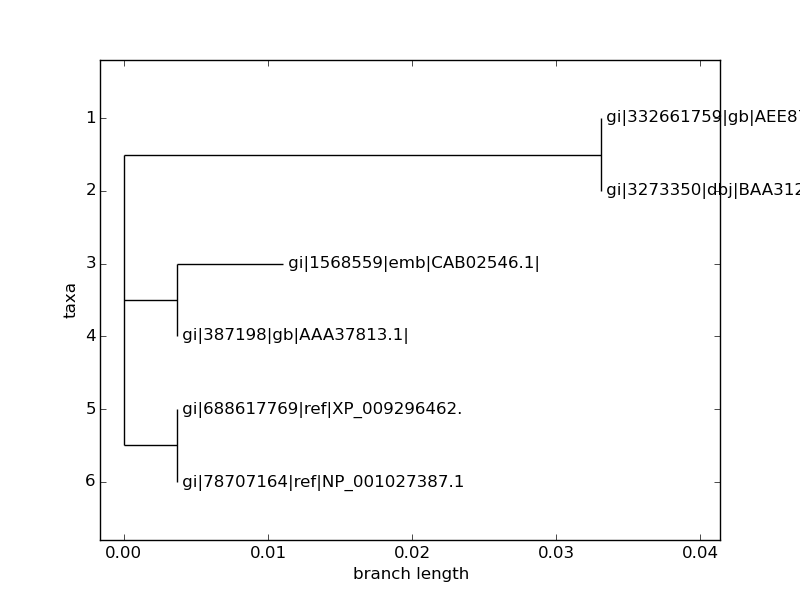
\includegraphics[width=0.45\textwidth]{h3-clustalw.png}
  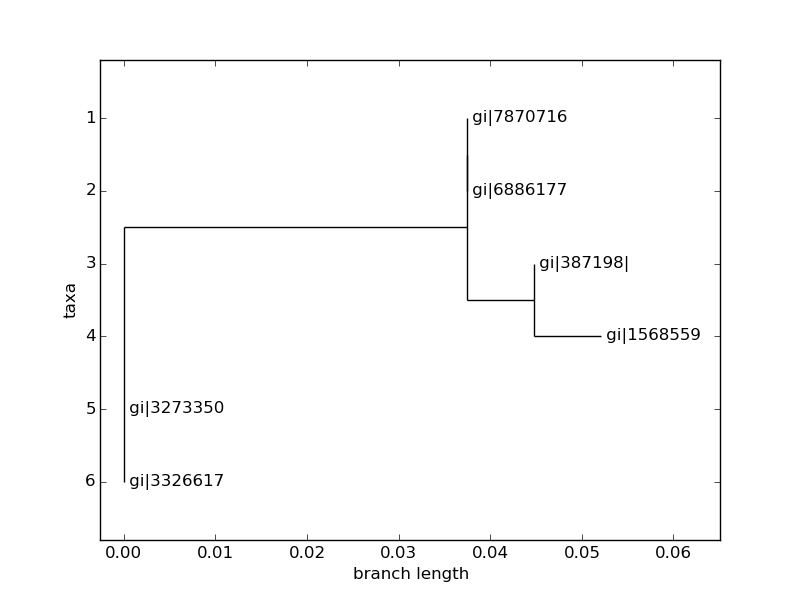
\includegraphics[width=0.45\textwidth]{h3-phyml.png}
  \caption{ClustalW tree on left for H3, Phyml tree on right. 332-Arabidopsis,
    156-human, 688-zebrafish,387-mouse, 787-drosophila melanogaster, 327-tobacco.}
\end{figure}

Phyml Tree:
\begin{verbatim}
(((gi|7870716:0.000000,gi|6886177:0.000000):0.000000,(gi|387198|:0.000000,gi|1568559:0.007289)
:0.007228):0.036831,gi|3273350:0.000000,gi|3326617:0.000000);
\end{verbatim}

ClustalW Tree:
\begin{verbatim}
((gi|332661759|gb|AEE87159.1|:0.00000,gi|3273350|dbj|BAA31218.1|:0.00000):0.03309,
(gi|1568559|emb|CAB02546.1|:0.00735,gi|387198|gb|AAA37813.1|:0.00000):0.00368,
(gi|688617769|ref|XP_009296462.:0.00000,gi|78707164|ref|NP_001027387.1:0.00000):0.00368);
\end{verbatim}

The PhyML tree accurately groups the mammals together, then the other animals, then the plants.
However, ClustalW does a better job of grouping each specific group together (mammals, non-mammals,
plants). PhyML doesn't show flies, zebrafish being more related to mammals than each other,
which seems innaccurate. So in that regard PhyML does a better job. Although PhyML doesn't seem
to be generating a binary tree, whereas ClustalW does. This could be because PhyML has a minimum
threshold for grouping things together, whereas ClustalW just takes the most related things and
groups them without a threshold.\\

\textbf{b.)}

\begin{figure}[h!]
  \centering
  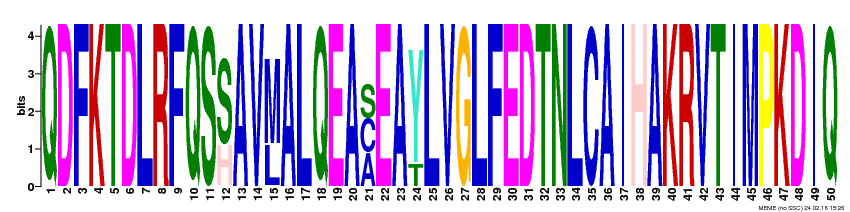
\includegraphics[width=0.75\textwidth]{oops-logo.png}\\
  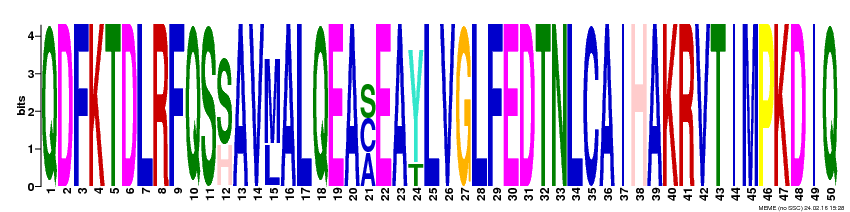
\includegraphics[width=0.75\textwidth]{anr-logo.png}
  \caption{OOPS on left, ANR on right.}
\end{figure}

These two found motifs in Figure 2 look almost identical. This suggests that there is only one
main motif in the sequences, so that one-occurence-per-sequence and any-number-of-occurrences
both finds the same number: one. If there were more motifs that met the motifness-threshold,
they would be found by ANR but not OOPS. The fact that there is only one main motif is plausible:
there is one active site on the coded protein, the rest of the protein is free to mutate to meet
the species' needs.\\

\section{Problem Three: More Trees}

\begin{figure}[h!]
  \centering
  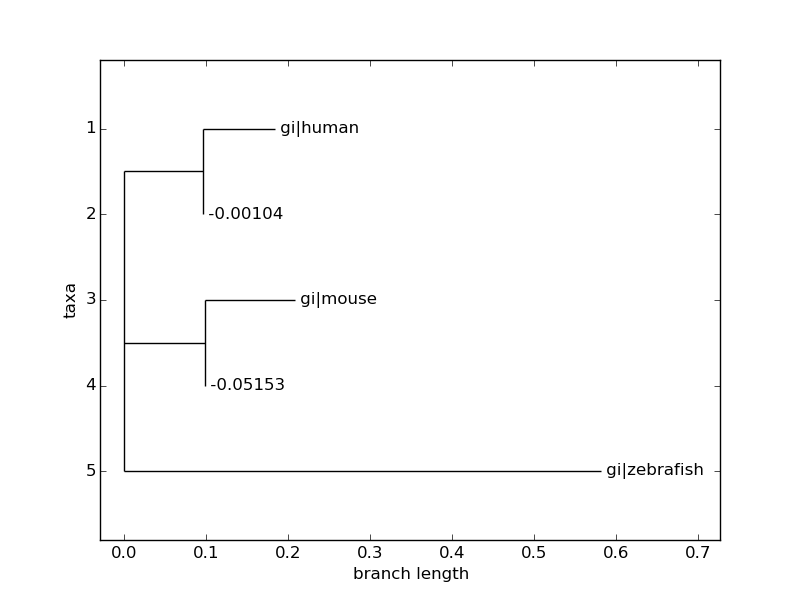
\includegraphics[width=0.45\textwidth]{clustalw.png}
  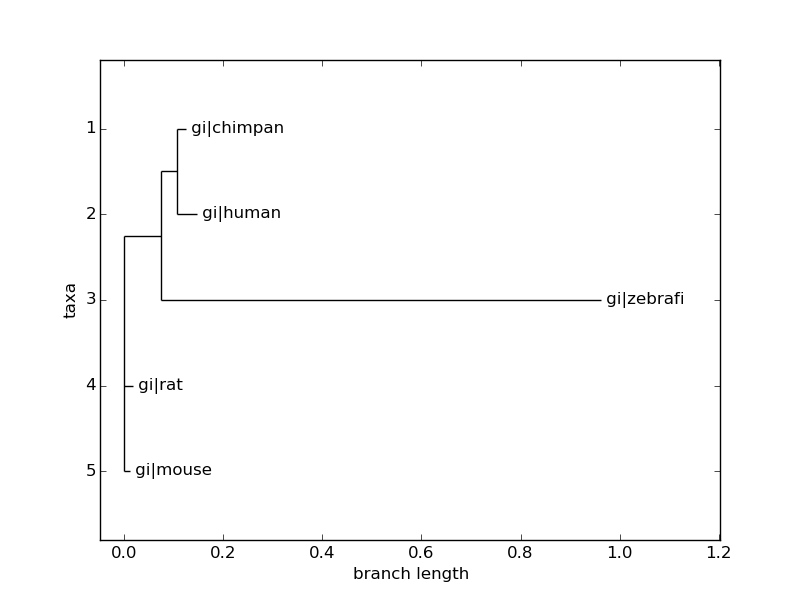
\includegraphics[width=0.45\textwidth]{phyml.png}
  \caption{ClustalW on left for HoxA, PhyML on right.}
\end{figure}

We see similar behavior here, where ClustalW insists on making a binary tree,
whereas PhyML does not. The trees look similar and seem to convey the same
information, which is good. It is interesting that zebrafish have such a
large distance from the other organisms. I guess it makes sense, since they
are an early type of fish? Plus the mRNA sequence for the zebrafish was much shorter
than the other sequences.\\

ClustalW Newick:
\begin{verbatim}
((gi|human:0.08731,gi|chimpanzee:-0.00104):0.09698,
(gi|mouse:0.10978,gi|rat:-0.05153):0.09846,gi|zebrafish:0.58169);
\end{verbatim}

PhyML Newick:
\begin{verbatim}
(((gi|chimpan:0.017786,gi|human:0.039499):0.032820,gi|zebrafi:0.886506)
:0.075342,gi|rat:0.019008,gi|mouse:0.012854);
\end{verbatim}

\section{Four: BED, GFF}

\textbf{a.)}\\
chr1 72 145 region1 100 + $\rightarrow$ chr1 progname feature 73 145 100 +\\
chr1 221 342 region2 100 + $\rightarrow$ chr1 progname feature 222 342 100 +\\
chr1 473 577 region3 100 + $\rightarrow$ chr1 progname feature 474 577 100 +\\

Here progname, feature are the names of the generating program and feature,
as BED does not specify them.\\

\textbf{b.)}\\
chr1 myDB gene 743 1200 . + . ID=gene1 $\rightarrow$ chr1 742 1200 name . +\\
chr1 myDB gene 3405 5345 . + . ID=gene2 $\rightarrow$ chr1 3404 5345 name . +\\
chr3 myDB mRNA 9143 9778 . + . ID=transcript1 $\rightarrow$ chr1 9142 9778 name . +\\

\section{Problem Five: Stalling Indices}

\textbf{Pol II Chip Tissue 2:}\\
We find the median of the gene body {1.1, 1.1, 1.1, 1.5, 1.7} to be 1.1.
We find the max $\pm$ 100 of the TSS to be 1.3 by inspection.\\
\begin{align*}
  SI = \frac{Max}{Median} &= \frac{1.3}{1.1} \approx 1.18
\end{align*}

\textbf{Pol II Chip Tissue 1:}\\
We find the median of {1.3, 1.3, 1.3, 1.5, 1.5} to be 1.3 and the max within 100pm of
the TSS to be 5.1 by inspection.\\
\begin{align*}
  SI = \frac{Max}{Median} &= \frac{5.1}{1.3} \approx 3.92
\end{align*}

\end{document}
